\section{Neural Networks}
\label{sec:NN}
Neural Networks (NN) are probably the most popular machine learning algorithms that we use today. This is also what is often used for face and speech recognition by companies like Google and Apple \cite{NNarticle}. NN does basically the same as a BDT, but instead of splitting the input data into background and signal at each node, each node is trained on different features. 

NN are a collection of nodes, like the ones we have in BDT. \ref{sec:BDT}. Instead of many trees with nodes, we create a network with these nodes as we can see in figure \ref{fig:NN}. 


\begin{figure}[H]
    \centering
    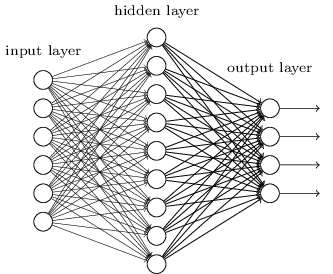
\includegraphics[width = 0.5\textwidth]{Figures/FromOnline/tikz35.png}
    \caption{Illustration of a neural network \cite{NNpic}.}
    \label{fig:NN}
\end{figure}

The network consists of one input layer, one hidden layer and one output layer. This is a very simple NN and is often called a \textit{shallow neural network} (SNN) since it has only one hidden layer. If we increase the number of hidden layers to two or more we have a deep neural network (DNN) as we can see in figure \ref{fig:DNN}

\begin{figure}[H]
    \centering
    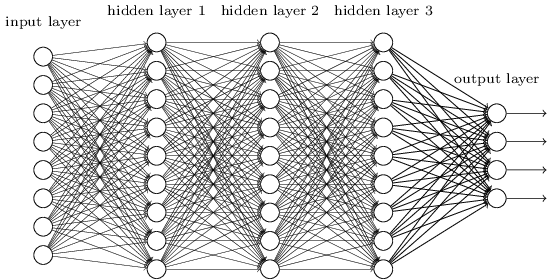
\includegraphics[width = 0.7\textwidth]{Figures/FromOnline/tikz36.png}
    \caption{Illustration of a deep neural network \cite{NNpic}.}
    \label{fig:DNN}
\end{figure}

In this thesis we have built a NN with a tool called \texttt{KerasClassifier}\footnote{Keras \cite{keras} is a NN library for Python.} which, as for the BDT, classifies the data. For our network to be able classify, we have to send in some pre-labeled data to train it. This is done by simply giving the background label 0 and signal label 1. Additionally, we have to understand what happens in the NN to know what parameters we should adjust in order to train and analyse the data. 

The NN has many more dependencies than the BDT. It is therefore unfortunately more sensitive to possible under- and overtraining, but for correct composition of parameters, it will typically be better trained than a BDT. To achieve the optimal results, we need a lot of computing power and time to optimize. 

There are many advantages and disadvantages with both SNN and DNN but it is in principle possible to achieve the same results with both. In a SNN you can increase the number of nodes and get the same results as for a DNN with several layers and fewer nodes in each layer. The problem with doing it that way is that we get more free parameters by increasing the number of nodes, which again increases the possibility that our model gets biased and hence over or underfits.

This is unfortunately not as trivial as for a BDT, but maybe easier to adapt to different purposes. In our case we are going to use it to distinguish signal from background.

With the basics in place, we can now describe NNs in more detail. Next we provide an overview of the activation function, how the network evolves, and how it gets better with training.

\subsection{Activation functions}
To get the output for the different nodes in a layer, we need an activation function. This output is again used as input for the next layer until you reach the last layer, which then will give us our final output/results.

Since Machine Learning doesn't come from a theoretical prediction which is implemented numerically, the choice of activation function for different problems is found by trial and error. The activation function will provide a number between 0 and 1 \cite{AF}, which is sent into the next nodes in the next layer. Some activation functions provide a number between -1 and 1 instead, but this depends on how the activation function we choose behaves, as we can see in figure \ref{fig:activations}. In the next sections we are going to look more closely at the different activation functions we have used in this thesis. We are also going to consider some other activation functions that are not used in this thesis but still of very common use in ML.


%In the network, each node uses an activation function to send the total input in that node as a number between 0 and 1 to the next layer. Tanh gives a number between -1 and 1.

\begin{figure}[H]
    \centering
    \begin{subfigure}[t!]{0.3\textwidth}
    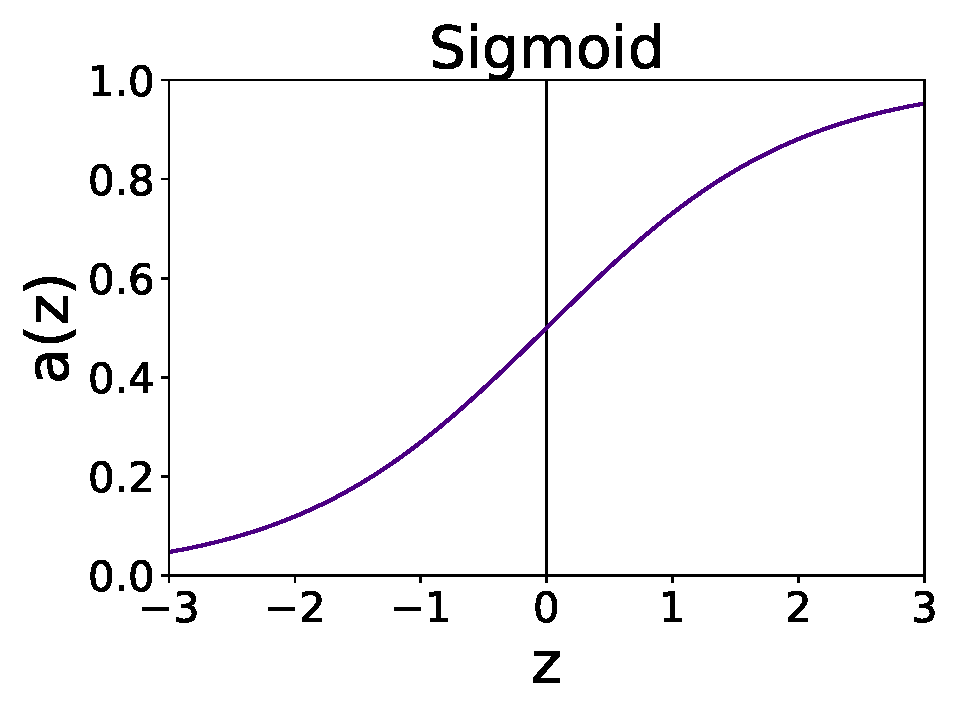
\includegraphics[width=\textwidth]{Figures/sigmoid.pdf}
    \caption{}
    \label{fig:sigmoid}
    \end{subfigure}
    \begin{subfigure}[t!]{0.3\textwidth}
    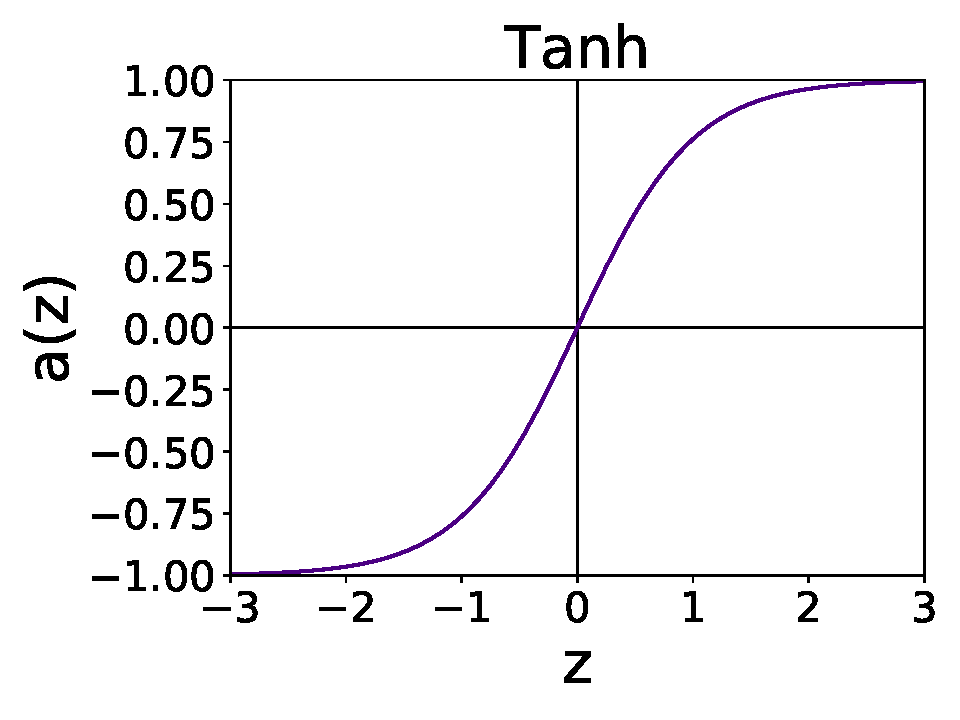
\includegraphics[width=\textwidth]{Figures/tanh.pdf}
    \caption{}
    \label{fig:tanh}
    \end{subfigure}
    \begin{subfigure}[t!]{0.3\textwidth}
    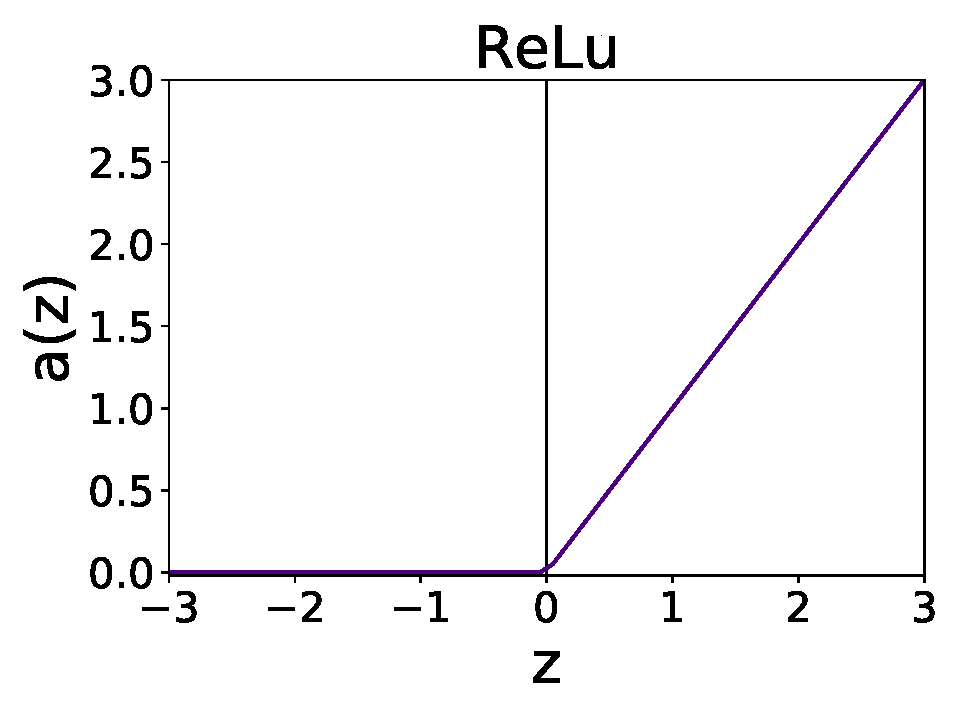
\includegraphics[width=\textwidth]{Figures/relu.pdf}
    \caption{}
    \label{fig:relu}
    \end{subfigure}
    \caption{This is an illustration of the behaviour of three different activation functions. In (a) we can see the Sigmoid function, in (b) the Tanh function, and in (c) the ReLU function.}
    \label{fig:activations}
\end{figure}



\textbf{Sigmoid}

The Sigmoid function, figure \ref{fig:sigmoid}, is a logistic activation function and is given by equation \ref{eq:sigmoid} below.

\begin{equation}
    \label{eq:sigmoid}
    a_i = \frac{1}{1+e^{(-z_i)}},
\end{equation}

where $z_i$ is the output value from the i-th node in the output layer.

As we can see in figure \ref{fig:sigmoid}, the Sigmoid function gives us a value between 0 and 1. This makes this activation function a good choice if we have to predict a probability for the output. A drawback, and the reason we have to use other activation functions sometimes, is that the Sigmoid can get the NN stuck on its training time because of the calculation time of the exponential. This is not an optimal activation function to use inside the network, but in the output layer it is the preferred one. We want our network to classify our output as signal or background which we have labeled as 1 and 0. 


\textbf{Tanh (Hyperbolic tangent)}

In addition to the Sigmoid function we have the tanh function, figure \ref{fig:tanh}, which is shaped the same way as the Sigmoid function, but it gives values between -1 and 1 instead of between 0 and 1. This we can see in figure \ref{fig:tanh} and it is given by equation \ref{eq:tanh} below.

\begin{equation}
\label{eq:tanh}
a_i = \tanh(z_i)
\end{equation}

Since we also can get negative numbers from this activation function, it is preferred instead of the Sigmoid if we have negative numbers in the input. This function returns negative values as negative unlike e.g. Sigmoid which only returns 0 or 1. Since we don't care for negative values in our case, this activation function is not used in this thesis. 

\textbf{ReLU (Rectified Linear Unit)}

One of the most popular activation functions is the ReLU function. This function outputs 0 for any negative value, and if the value is positive, the function returns the value as it is. This is shown in figure \ref{fig:relu}. Since all data that is below zero becomes zero, it can be hard do get a good read out of the data because the data may sometimes assume negative values. The ReLU function is given by equation \ref{eq:relu}.

\begin{equation}
\label{eq:relu}
    a_i = max(0,z_i).
\end{equation}

Since we're not interested in negative values we are using this activation function in our hidden layers. The Sigmoid function would also be a good choice when we are thinking about our wanted form of the output. But, as mentioned earlier, it can get stuck in its training time.

\textbf{Other activation functions}

The three functions mentioned above are not the only activation functions one can use. Since every problem has different approaches, we have to adjust these functions for our needs. There are, for example, many different adjustments done with the ReLU function to get a better activation output in problems that need adjustment to perform optimally. One of the newest activation functions is called Swish \cite{Swish}, which is simply a modification of the Sigmoid function given by equation \ref{eq:swish}. 

\begin{equation}
    \label{eq:swish}
    a(x) = x \cdot Sigmoid(x)
\end{equation}

The developers of the Swish function state that it does overall a better job than the widely used ReLU function, but until this time there is no evidence in literature supporting this claim. As such, we will stick with ReLU in this thesis. 

\subsection{Feed forward and back propagation} 
Every node in the neural network has an activation function connected to itself and if the node is connected to another node it also has a weight for each node it is connected to. To create the new node we simply multiply the nodes activation with the weight and sum them together like so

\begin{equation}
    a_1 \cdot w_1 + .. + a_n \cdot w_n = \text{new node}
\end{equation}

This operation is done for every node in every layer, and fed to the next layer until we hit the the output layer. This is what we call \textit{feed forward} because we always send the obtained information forward from input to output layer.

We also have a method to go back in the network to optimize it, namely \textit{back propagation}. What we do is go back to the previous layers to optimize the weights. This is not what we call an optimizer and should not be confused with that; it's merely the process of going backwards. Back propagation is probably the most important step in a NN, because this optimizes our model and makes sure that our training goes well. 

\subsection{Optimizers}

When training a NN, we need to know how well it performs during and after the training. For this we use a loss function $L$. There are many different types of functions that are used, depending on what we want to do with the network.

We want to minimize the loss function to make the prediction error as small as possible, i.e. optimize the network. And to do this, we use an optimizer.

\subsubsection{Stochastic Gradient Descent\cite{training_model}}

The gradient descent method uses the fact that a function $F(x)$, where $x = (x_1,x_2,...,x_n)$, will increase fastest in the direction of the gradient of the function, $\nabla F$. We want to move in the opposite direction of the gradient to make sure that we decrease the loss function.

We then multiply this gradient with a number $\eta$ called "the learning rate", and subtract this from the current weights $w_j$. In the case of neural networks, $F(x)$ is the loss function $L$. This leads to equation \ref{eq:w_update} 

\begin{equation}
    w_j = w_j - \eta\frac{\partial L}{\partial w_j}
    \label{eq:w_update}
\end{equation}

To speed up the training we can also add a stochastic part to the method, which means that we randomly choose a batch size of the data that we use to approximate the derivative, and use that to update the weights. This is also called Mini Batch Gradient Descent. 

The data that we want to use might be very noisy, so we can use a technique to de-noise the data \cite{SGD_momentum}. This is done by adding a momentum, which is a moving average of our gradients. We now subtract this from the weights. The equations now become 

\begin{equation}
    V_i = \beta V_i + (1 - \beta)\nabla_w L
    w_i = w_i - \eta V_i
    \label{eq:momentum}
\end{equation}

One way to look at this last addition is viewing the movement in parameter space as an object that moves one step at a time downhill. When we add momentum, it is like giving this object some physical momentum. Now when the object finds the minimum, it will continue a little bit back and forth to make sure it has found the minimum. A good reason to add this is if there are many saddle-points where the optimizer might stop. With momentum, it will move past, and then continue the descent on the other side without stopping.

\subsubsection{Adam\cite{Goodfellow-et-al-2016}}

The learning rate is one of the most difficult parameters to optimize, because any change to its value may have a huge impact on a method's performance. To circumvent this, we can use a method that has an adaptive learning rate. 

Adam is currently the most popular optimization algorithm today, and the name is derived from Adaptive Moments. It is an update to another optimization algorithm called RMSProp, which stands for Root Mean Square Propagation. RMSProp uses the running average of recent gradient magnitudes, and divides the learning rate by this average. This is done for every weight in the NN.

Adam takes this a step further. It uses an estimation of the first-order moments of the gradient as momentum, and also adds a bias correction to both the momentum and the second-order moments.

